\documentclass[tikz,border=1.25mm]{standalone}
\usetikzlibrary{matrix, positioning, shapes, fit, shapes.geometric, backgrounds, arrows.meta}
\usepackage{amssymb}

\definecolor{kellygreen}{rgb}{0.3, 0.73, 0.09}
\definecolor{gray}{rgb}{0.54, 0.54, 0.54}
\definecolor{slate}{rgb}{0.094,0.094,0.094}
\definecolor{cobalt}{rgb}{0.244,0.364,0.972}

\begin{document}

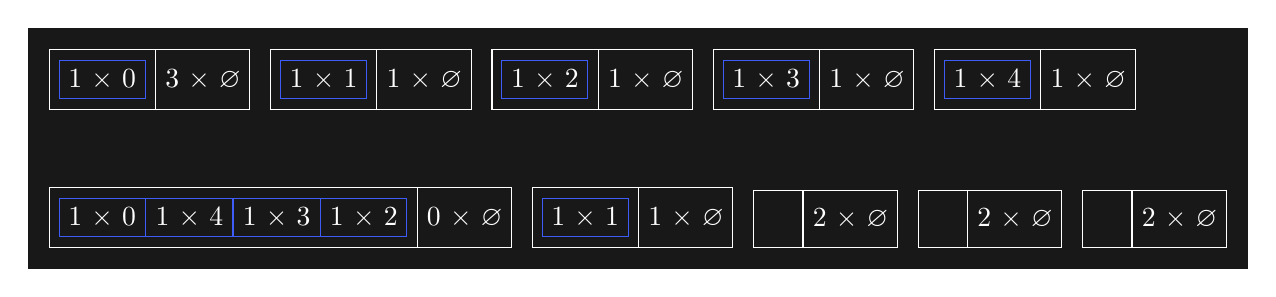
\begin{tikzpicture}[
  background rectangle/.style={fill=slate},
  show background rectangle,
  every node/.style={
    color=white,
    draw,
    minimum height=4.6mm,
  }
]

\matrix(m0)[
    matrix anchor=north west,
    matrix of nodes,
	nodes in empty cells,
	column sep=2.5mm,
	row sep=5mm,
	draw=none
] {
\node[rectangle split, rectangle split horizontal, rectangle split parts=2, draw]{
    \nodepart{one} \tikz{\node[rectangle split, rectangle split horizontal, rectangle split parts=1, draw, color=cobalt, text=white]{
        \nodepart{one} 1 $\times$ 0
    }}
    \nodepart{two} 3 $\times$ $\varnothing$
  }; &
  \node[rectangle split, rectangle split horizontal, rectangle split parts=2, draw]{
    \nodepart{one} \tikz{\node[rectangle split, rectangle split horizontal, rectangle split parts=1, draw, color=cobalt, text=white]{
        \nodepart{one} 1 $\times$ 1
    }}
    \nodepart{two} 1 $\times$ $\varnothing$
  }; &
  \node[rectangle split, rectangle split horizontal, rectangle split parts=2, draw]{
    \nodepart{one} \tikz{\node[rectangle split, rectangle split horizontal, rectangle split parts=1, draw, color=cobalt, text=white]{
        \nodepart{one} 1 $\times$ 2
    }}
    \nodepart{two} 1 $\times$ $\varnothing$
  }; &
  \node[rectangle split, rectangle split horizontal, rectangle split parts=2, draw]{
    \nodepart{one} \tikz{\node[rectangle split, rectangle split horizontal, rectangle split parts=1, draw, color=cobalt, text=white]{
        \nodepart{one} 1 $\times$ 3
    }}
    \nodepart{two} 1 $\times$ $\varnothing$
  }; &
  \node[rectangle split, rectangle split horizontal, rectangle split parts=2, draw]{
    \nodepart{one} \tikz{\node[rectangle split, rectangle split horizontal, rectangle split parts=1, draw, color=cobalt, text=white]{
        \nodepart{one} 1 $\times$ 4
    }}
    \nodepart{two} 1 $\times$ $\varnothing$
  }; \\
};

\matrix(m1)[
  matrix anchor=north west,
  below=17.5mm of m0.north west,
  matrix of nodes,
  nodes in empty cells,
  column sep=2.5mm,
  row sep=5mm,
  draw=none
] {
  \node[rectangle split, rectangle split horizontal, rectangle split parts=2, draw]{
    \nodepart{one} \tikz{\node[rectangle split, rectangle split horizontal, rectangle split parts=4, draw, color=cobalt, text=white]{
        \nodepart{one} 1 $\times$ 0
        \nodepart{two} 1 $\times$ 4
        \nodepart{three} 1 $\times$ 3
        \nodepart{four} 1 $\times$ 2
    }}
    \nodepart{two} 0 $\times$ $\varnothing$
  }; &
  \node[rectangle split, rectangle split horizontal, rectangle split parts=2, draw]{
    \nodepart{one} \tikz{\node[rectangle split, rectangle split horizontal, rectangle split parts=1, draw, color=cobalt, text=white]{
        \nodepart{one} 1 $\times$ 1
    }}
    \nodepart{two} 1 $\times$ $\varnothing$
  }; &
  \node[rectangle split, rectangle split horizontal, rectangle split parts=2, draw]{
    \nodepart{one} \tikz{\node[rectangle split, rectangle split horizontal, rectangle split parts=1, draw=none]{}}
    \nodepart{two} 2 $\times$ $\varnothing$
  }; &
  \node[rectangle split, rectangle split horizontal, rectangle split parts=2, draw]{
    \nodepart{one} \tikz{\node[rectangle split, rectangle split horizontal, rectangle split parts=1, draw=none]{}}
    \nodepart{two} 2 $\times$ $\varnothing$
  }; &
  \node[rectangle split, rectangle split horizontal, rectangle split parts=2, draw]{
    \nodepart{one} \tikz{\node[rectangle split, rectangle split horizontal, rectangle split parts=1, draw=none]{}}
    \nodepart{two} 2 $\times$ $\varnothing$
  }; \\
};

\end{tikzpicture}

\end{document}
